\documentclass[a4paper,12pt, oneside]{article}

\title{\textbf{L'impatto del Codec AV1 sull'industria della visualizzazione online} \\ \large A.A 2023/2024 \\ Elaborato di Crittografia}
\author{Gabos Norbert \\ 0000970451 \\ tiberiunorbert.gabos@studio.unibo.it }
\date{}

\usepackage[T1]{fontenc}
\usepackage[utf8]{inputenc}
\usepackage[italian]{babel}
\pagestyle{plain}
\usepackage{graphicx}
\usepackage[table,xcdraw]{xcolor}
\usepackage{tabularx}
\usepackage{ragged2e}               % migliora la formattazione del testo all'interno delle celle
\renewcommand{\arraystretch}{1.5}   % aggiunge margine alle celle
\graphicspath{{images/}}

\definecolor{darkBlue}{RGB}{21, 69, 179}
\definecolor{lightPink}{RGB}{242, 10, 172}

\begin{document}

\maketitle

\newpage
\tableofcontents{}
\newpage

\section{Introduzione}
Con l'avvento dei computer e la crescente digitalizzazione dei media, è emersa la necessità di
trovare soluzioni efficaci per rappresentare e archiviare i video all'interno dei sistemi
informatici. Questo processo ha comportato la trasformazione dei tradizionali filmati in una
forma compatibile con il mondo digitale, dove ogni istante del video è rappresentato da una
sequenza di immagini statiche, comunemente note come frame. Ogni frame, a sua volta, è
composto da una matrice di pixel, gli elementi fondamentali che compongono l'immagine, ognuno
dei quali è definito da una terna di colori \textbf{RGB} (Red, Green, Blue) e da una profondità
di colore che varia generalmente tra 0 e 255.

Questo approccio ha permesso di preservare la qualità visiva dei contenuti video e di renderli
compatibili con le capacità di elaborazione dei computer. Tuttavia, la mera rappresentazione
dei video in questo modo ha portato ad un'elevata quantità di dati da gestire ed archiviare
comportando sfide significative in termini di spazio di archiviazione e larghezza di banda.
Per esempio un banale video da 10 minuti in 1080p a 30 fotogrammi al secondo pesa
all'incirca 111 GB.
\noindent
\\\\Peso\_video = Risoluzione × Fotogrammi\_al\_secondo × Durata × Profondità\_colore\\

Nei primi anni '80, con il crescente bisogno di gestire file video in un contesto di limitate
capacità di archiviazione, si svilupparono i primi \textbf{codec} video. Questi non solo consentivano
la compressione dei file video, ma anche la decodifica. Questo rappresentava una soluzione
importante, poiché i dispositivi dell'epoca potevano immagazzinare solo una quantità limitata
di dati, mentre le esigenze di qualità video e il numero di dispositivi produttori di contenuti
multimediali aumentavano costantemente.
Per affrontare queste sfide e ottimizzare l'archiviazione e la trasmissione dei video
digitali, sono stati sviluppati una serie di algoritmi e standard di compressione video.
Esistono due approcci principali alla compressione video: la compressione \textbf{lossless} e
la compressione \textbf{lossy}. La compressione lossless, ad esempio con algoritmi come
\textbf{Huffyuv} e \textbf{Lagarith}, mira a ridurre le dimensioni del file senza perdita di
qualità, mantenendo ogni singolo dato originale. D'altro canto, la compressione lossy
sacrifica una certa quantità di qualità visiva per raggiungere una maggiore compressione dei
dati, consentendo una gestione più efficiente delle risorse di archiviazione e una
trasmissione più rapida attraverso le reti digitali.

In questa relazione, esploreremo l'evoluzione della compressione video lossy, partendo dal
contesto della sua necessità fino alla discussione di algoritmi più recenti e avanzati come il
Codec AV1. Analizzeremo come questi algoritmi hanno rivoluzionato il modo in cui i video
vengono elaborati, archiviati e trasmessi sui mezzi digitali, con un focus particolare sugli
impatti e le potenzialità di tali innovazioni nell'industria multimediale moderna.

\section{I primi passi}
\subsection{H.261}
Nel 1988 nasce il codec H261 che è stato il primo algoritmo di compressione video ad utilizzare
in modo efficiente degli algoritmo di \textbf{intraframe} e \textbf{interframe}, che sono
spiegati nel capitolo successivo, ed è responsabile dell'introduzione della codifica video
ibrida basata su blocchi, che è ancora utilizzata oggi in molti standard video.
\\\\Prima di proseguire, visto che non parliamo più dei video come una matrice di pixel, ma più di
un flusso di dati, bisogna introdurre il concetto di bitrate.
Il \textbf{bitrate} è una misura della velocità di trasmissione dei dati in un file multimediale,
come un video o un brano audio. Rappresenta quanti dati vengono trasmessi o elaborati in un
determinato intervallo di tempo espresso in \textbf{bit/s}. In generale, a parità di tecnologie
utilizzate per la compressione, più il bitrate di un contenuto è elevato e più la sua qualità
sarà maggiore al costo di un peso più elevato. Vedi Figura~\ref{fig:confronto_bitrate}.

\begin{figure}[h]
    \centering
    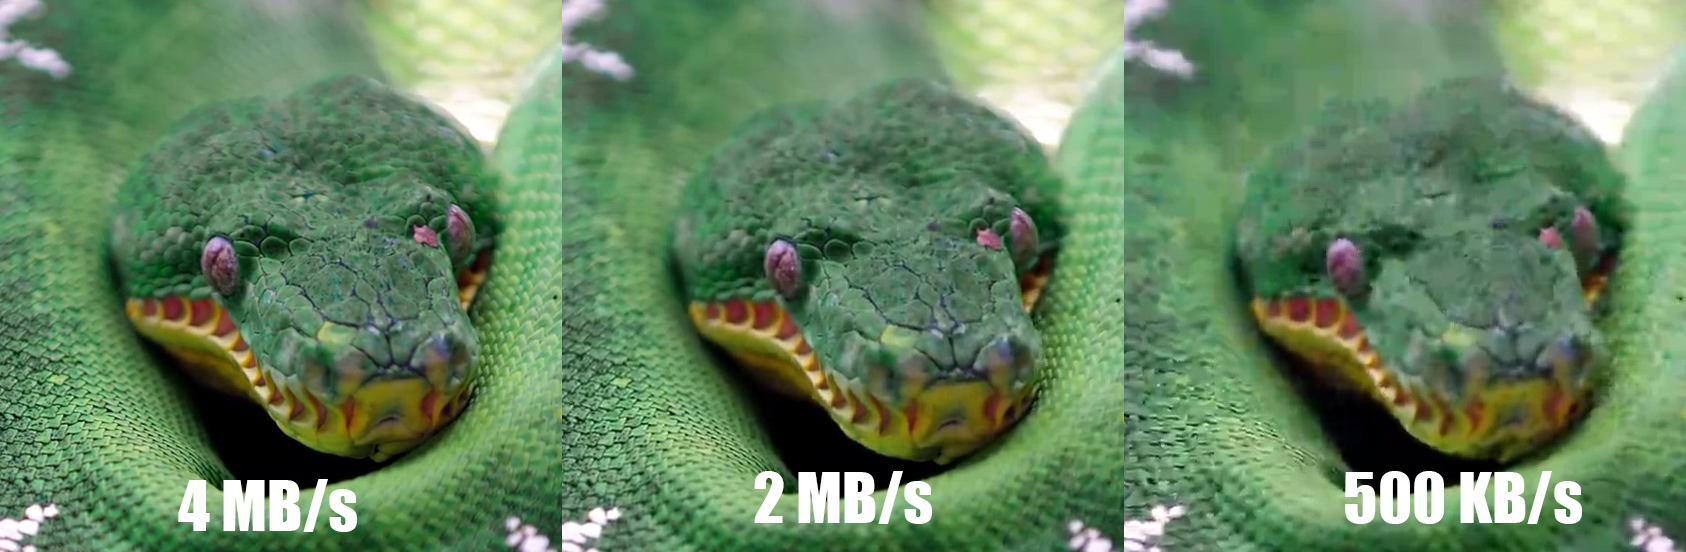
\includegraphics[width=1\textwidth]{images/confronto-bitrate.png}
    \caption{L'immagine mette a confronto 3 frame presi allo stesso istante da un video compresso con 3 valori di bitrate differenti.}
    \label{fig:confronto_bitrate}
\end{figure}

\noindent
Un aspetto sorprendente di questo algoritmo è che per rilevare una diminuzione nella qualità del
video, è necessario ridurre significativamente il bitrate.
Per fare un confronto con l'esempio di prima del video da 10 minuti, utilizzando questo codec potremmo
ridurre nettamente la dimensione del file anche di 300 volte. Usando un bitrate che varia dai 5-10 Mb/s,
quindi un bit rate elevato per questa risoluzione che ci permette di mantenere un'ottima qualità,
il file compresso avrebbe una dimensione dai 375 ai 750 MB.

\section{Tecnologie attuali}
\subsection{H.264/AVC}
Il formato H.264 è stato introdotto nel 2003 e appartiene alla serie H.26X. Il suo obiettivo principale
è quello di comprimere ulteriormente i file video senza compromettere la qualità visiva. Questa
tecnologia consente di ottenere file video più leggeri mantenendo comunque un'elevata qualità
dell'immagine. In alternativa, è possibile mantenere le stesse dimensioni dei file video ma migliorare
la qualità visiva. Questo codec sarà fondamentale anche in futuro con l'espansione dei servizi di
streaming in tempo reale. Ciò permetterà alle aziende di risparmiare sui costi delle infrastrutture
per l'archiviazione e la trasmissione dei dati via rete, e offrirà agli utenti finali con connessioni
internet di scarsa qualità la possibilità di fruire di questi servizi.

Nonostante siano trascorsi più di 20 anni dalla creazione del formato H.264, merita comunque attenzione
in virtù del suo status di standard rivoluzionario nella codifica video. Nel settembre 2019, ha
raggiunto un notevole 91\% di adozione tra gli sviluppatori nel settore video, confermandosi così come
un pilastro fondamentale della tecnologia di compressione video. Inoltre, alcune delle tecnologie
adottate da questo codec saranno cruciali per comprendere meglio il funzionamento dei codec successivi.

\paragraph{Macroblock}\hphantom{A}\\
TODO

\paragraph{Intraframe/intra prediciton}\hphantom{A}\\
\begin{figure}[h]
    \centering
    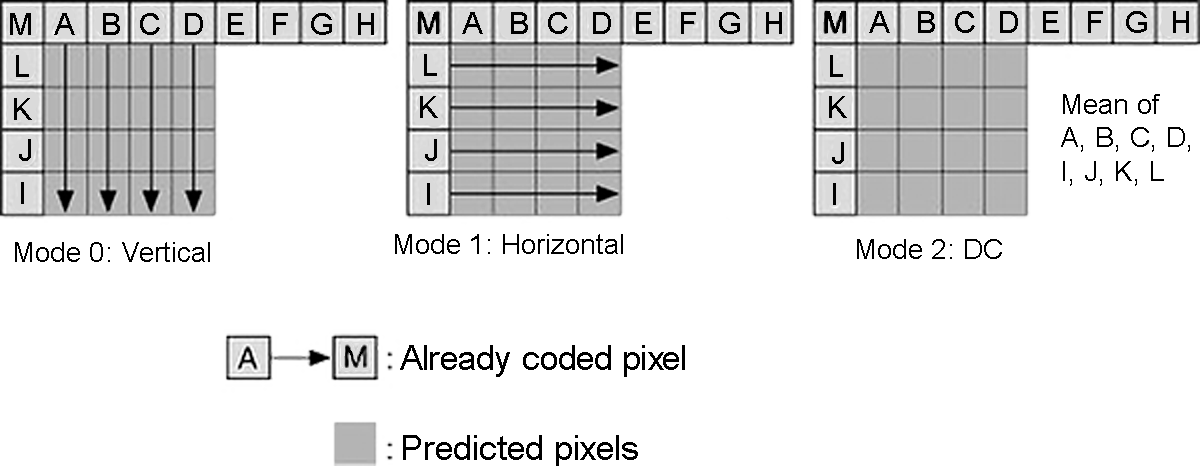
\includegraphics[width=1\textwidth]{images/intraframe-algo.png}
    \caption{Rappresentazione dei 3 metodi più utilizzati per la predizione intraframe}
    \label{fig:intraframe_algo}
\end{figure}
La compressione intraframe, si riferisce alla compressione dei dati all'interno di un singolo
fotogramma. Questo metodo si divide più passaggi:
\begin{enumerate}
  \item Per ogni macroblock, viene utilizzato un modello di predizione per stimare i valori dei pixel
  all'interno del blocco basandosi sui valori dei pixel circostanti. Questo modello di predizione può
  essere semplice (come la predizione dei pixel adiacenti) o più complesso (come la predizione basata
  su modelli statistici o algoritmi di machine learning). I 3 metodi più utilizzati sono (Vedi
  Figura~\ref{fig:intraframe_algo}) : traslandolo i pixel adiacenti già noti in orizzontale/verticale
  oppure facendo una media dei pixel adiacenti.
  Nel caso del formato H.264 ci sono in totale 9 algoritmi di intraframe.
  \item Successivamente viene calcolata la residua, ovvero la differenza tra i pixel predetti e i
  pixel dell'immagine non compressa
  \item Infine viene scelta la matrice residua, che si è avvicinata di più al gruppo di pixel originale,
  comprimendo così la dimensione del frame.
\end{enumerate}

TODO: non so se inserire l'esempio (nel caso le immagini sono gia salvate)

\paragraph{Interframe}\hphantom{A}\\
La compressione interframe, lavora sulla
ridondanza temporale tra i frame adiacenti. Invece di codificare ogni frame singolarmente,
vengono identificate e codificate solo le differenze tra i frame successivi o precedenti.
Questo consente di ridurre ulteriormente le dimensioni del file video, poiché molte
informazioni rimangono costanti tra i fotogrammi vicini.

Il formato H.264 è stato anche il primo formato che necessitava di specifici acceleratori hardware per
poter decodificare i video in tempo reale in quanto i calcoli da eseguire iniziavano ad essere molto
complessi. Questo portò alla luce che con l'avanzare delle nuove tecnologie per la compressione dei
video, che riducevano le dimensioni dei file, aumentava anche la potenza di calcolo necessaria per
la codifica e decodifica dei video.

Introduce la possibilità di codificare fino a 4k, poi più avanti arriva fino all'8k.
Youtube lo ha usato fino al 2010 per poi abbandonarlo in favore del proprio VP8.
TODO: L'h264 essendo una tecnica che racchiude molti algoritmi complessi per la compressione video, necessita di accelleratori hardware per poter decodificare i fotogrammi in tempo reale.

\subsection{H.265}
Fino a 8K
\subsection{VP9}    % forse non serve descriverlo
\subsection{AV1}
TODO: il codec AV1 è molto lento nel codificare/decodificare video, ma con un accelleratore apposito è nettamente più volece del H.265

\subsection{Comparazione delle prestazioni}

\section{Vantaggi per le aziende}

\section{Sfide e considerazioni}
Non dimenticare di discutere anche delle sfide e delle considerazioni pratiche legate all'adozione di nuovi codec, come il supporto hardware/software, la compatibilità con dispositivi esistenti e la gestione dei diritti d'autore.

\section{Conclusioni}
TODO: si potrbbe parlare dell'approccio di NVIDIA per le video chat.

\section{Bibliografia}
\\+sito che parla della storia degli encorder https://api.video/blog/video-trends/the-history-of-video-compression-starts-in-1929/
\\+parla dei tecnicismi del h.261 https://users.ece.utexas.edu/~ryerraballi/MSB/pdfs/M4L2.pdf
\\+bitrate https://it.wikipedia.org/wiki/Velocit%C3%A0_di_trasmissione
\\-utile! parla dei tecnicismi del h.264 nella sezione di Implementing h.264 https://www.embedded.com/implementing-h-264-video-compression-\\algorithms-on-a-software-configurable-processor/
\\+utile! intra prediction https://www.sciencedirect.com/topics/computer-science/intra-prediction
\\-utile! sito di International Telecommunication Union che parla dello standard h.264 https://www.itu.int/rec/T-REC-H.264-202108-I/en
\\+repository di un'implementazione dell'h.264 https://github.com/cisco/openh264
\\-sito ufficiale di h.265 https://hevc.hhi.fraunhofer.de/
\\+repository di h.265 https://vcgit.hhi.fraunhofer.de/jvet/HM
\\-utile! parla dei tecnicismi del h.265 nella sezione di Coding tools https://en.wikipedia.org/wiki/High_Efficiency_Video_Coding
\\-utile! paragona AV1 a h.265 https://subclassy.github.io/compression#:~:text=265%20takes%202.83s%20on,so%20much%20time%20to%20process.
\\-utile! paragona le performance dei vari codec su hw nvidia https://developer.nvidia.com/video-codec-sdk
\\-utile! https://support.google.com/youtube/answer/2853702?hl=it

\end{document}
